% !TEX TS-program = pdflatex
% !TEX encoding = UTF-8 Unicode

% This is a simple template for a LaTeX document using the "article" class.
% See "book", "report", "letter" for other types of document.


\documentclass[11pt]{article} % use larger type; default would be 10pt

\usepackage[utf8]{inputenc} % set input encoding (not needed with XeLaTeX)
\usepackage{graphicx}
\graphicspath{ {figures/} }
\usepackage{array}

%%% Examples of Article customizations
% These packages are optional, depending whether you want the features they provide.
% See the LaTeX Companion or other references for full information.

%%% PAGE DIMENSIONS
\usepackage{geometry} % to change the page dimensions
\geometry{letterpaper} % or letterpaper (US) or a5paper or....
% \geometry{margin=2in} % for example, change the margins to 2 inches all round
% \geometry{landscape} % set up the page for landscape
%   read geometry.pdf for detailed page layout information

\usepackage{graphicx} % support the \includegraphics command and options

% \usepackage[parfill]{parskip} % Activate to begin paragraphs with an empty line rather than an indent

%%% PACKAGES
\usepackage{booktabs} % for much better looking tables
\usepackage{array} % for better arrays (eg matrices) in maths
\usepackage{paralist} % very flexible & customisable lists (eg. enumerate/itemize, etc.)
\usepackage{verbatim} % adds environment for commenting out blocks of text & for better verbatim
\usepackage{subfig} % make it possible to include more than one captioned figure/table in a single float
% These packages are all incorporated in the memoir class to one degree or another...

%%% HEADERS & FOOTERS
\usepackage{fancyhdr} % This should be set AFTER setting up the page geometry
\pagestyle{fancy} % options: empty , plain , fancy
\renewcommand{\headrulewidth}{0pt} % customise the layout...
\lhead{}\chead{}\rhead{}
\lfoot{}\cfoot{\thepage}\rfoot{}

%%% SECTION TITLE APPEARANCE
\usepackage{sectsty}
\allsectionsfont{\sffamily\mdseries\upshape} % (See the fntguide.pdf for font help)
% (This matches ConTeXt defaults)

%%% ToC (table of contents) APPEARANCE
\usepackage[nottoc,notlof,notlot]{tocbibind} % Put the bibliography in the ToC
\usepackage[titles,subfigure]{tocloft} % Alter the style of the Table of Contents
\renewcommand{\cftsecfont}{\rmfamily\mdseries\upshape}
\renewcommand{\cftsecpagefont}{\rmfamily\mdseries\upshape} % No bold!
\usepackage{float}
\usepackage{amsmath}
 %%%%%%%%%%%%%%%%%%%%%%%%%%%%%%%%%%%%%%%%%%%%%%%%%%%%%%%%%%%%%%%%%%%%%%%%%%%%%%%% 
%%% ~ Arduino Language - Arduino IDE Colors ~                                  %%%
%%%                                                                            %%%
%%% Kyle Rocha-Brownell | 10/2/2017 | No Licence                               %%%
%%% -------------------------------------------------------------------------- %%%
%%%                                                                            %%%
%%% Place this file in your working directory (next to the latex file you're   %%%
%%% working on).  To add it to your project, place:                            %%%
%%%     %%%%%%%%%%%%%%%%%%%%%%%%%%%%%%%%%%%%%%%%%%%%%%%%%%%%%%%%%%%%%%%%%%%%%%%%%%%%%%%% 
%%% ~ Arduino Language - Arduino IDE Colors ~                                  %%%
%%%                                                                            %%%
%%% Kyle Rocha-Brownell | 10/2/2017 | No Licence                               %%%
%%% -------------------------------------------------------------------------- %%%
%%%                                                                            %%%
%%% Place this file in your working directory (next to the latex file you're   %%%
%%% working on).  To add it to your project, place:                            %%%
%%%     %%%%%%%%%%%%%%%%%%%%%%%%%%%%%%%%%%%%%%%%%%%%%%%%%%%%%%%%%%%%%%%%%%%%%%%%%%%%%%%% 
%%% ~ Arduino Language - Arduino IDE Colors ~                                  %%%
%%%                                                                            %%%
%%% Kyle Rocha-Brownell | 10/2/2017 | No Licence                               %%%
%%% -------------------------------------------------------------------------- %%%
%%%                                                                            %%%
%%% Place this file in your working directory (next to the latex file you're   %%%
%%% working on).  To add it to your project, place:                            %%%
%%%    \input{arduinoLanguage.tex}                                             %%%
%%% somewhere before \begin{document} in your latex file.                      %%%
%%%                                                                            %%%
%%% In your document, place your arduino code between:                         %%%
%%%   \begin{lstlisting}[language=Arduino]                                     %%%
%%% and:                                                                       %%%
%%%   \end{lstlisting}                                                         %%%
%%%                                                                            %%%
%%% Or create your own style to add non-built-in functions and variables.      %%%
%%%                                                                            %%%
 %%%%%%%%%%%%%%%%%%%%%%%%%%%%%%%%%%%%%%%%%%%%%%%%%%%%%%%%%%%%%%%%%%%%%%%%%%%%%%%% 

\usepackage{color}
\usepackage{listings}    
\usepackage{courier}

%%% Define Custom IDE Colors %%%
\definecolor{arduinoGreen}    {rgb} {0.17, 0.43, 0.01}
\definecolor{arduinoGrey}     {rgb} {0.47, 0.47, 0.33}
\definecolor{arduinoOrange}   {rgb} {0.8 , 0.4 , 0   }
\definecolor{arduinoBlue}     {rgb} {0.01, 0.61, 0.98}
\definecolor{arduinoDarkBlue} {rgb} {0.0 , 0.2 , 0.5 }

%%% Define Arduino Language %%%
\lstdefinelanguage{Arduino}{
  language=C++, % begin with default C++ settings 
%
%
  %%% Keyword Color Group 1 %%%  (called KEYWORD3 by arduino)
  keywordstyle=\color{arduinoGreen},   
  deletekeywords={  % remove all arduino keywords that might be in c++
                break, case, override, final, continue, default, do, else, for, 
                if, return, goto, switch, throw, try, while, setup, loop, export, 
                not, or, and, xor, include, define, elif, else, error, if, ifdef, 
                ifndef, pragma, warning,
                HIGH, LOW, INPUT, INPUT_PULLUP, OUTPUT, DEC, BIN, HEX, OCT, PI, 
                HALF_PI, TWO_PI, LSBFIRST, MSBFIRST, CHANGE, FALLING, RISING, 
                DEFAULT, EXTERNAL, INTERNAL, INTERNAL1V1, INTERNAL2V56, LED_BUILTIN, 
                LED_BUILTIN_RX, LED_BUILTIN_TX, DIGITAL_MESSAGE, FIRMATA_STRING, 
                ANALOG_MESSAGE, REPORT_DIGITAL, REPORT_ANALOG, SET_PIN_MODE, 
                SYSTEM_RESET, SYSEX_START, auto, int8_t, int16_t, int32_t, int64_t, 
                uint8_t, uint16_t, uint32_t, uint64_t, char16_t, char32_t, operator, 
                enum, delete, bool, boolean, byte, char, const, false, float, double, 
                null, NULL, int, long, new, private, protected, public, short, 
                signed, static, volatile, String, void, true, unsigned, word, array, 
                sizeof, dynamic_cast, typedef, const_cast, struct, static_cast, union, 
                friend, extern, class, reinterpret_cast, register, explicit, inline, 
                _Bool, complex, _Complex, _Imaginary, atomic_bool, atomic_char, 
                atomic_schar, atomic_uchar, atomic_short, atomic_ushort, atomic_int, 
                atomic_uint, atomic_long, atomic_ulong, atomic_llong, atomic_ullong, 
                virtual, PROGMEM,
                Serial, Serial1, Serial2, Serial3, SerialUSB, Keyboard, Mouse,
                abs, acos, asin, atan, atan2, ceil, constrain, cos, degrees, exp, 
                floor, log, map, max, min, radians, random, randomSeed, round, sin, 
                sq, sqrt, tan, pow, bitRead, bitWrite, bitSet, bitClear, bit, 
                highByte, lowByte, analogReference, analogRead, 
                analogReadResolution, analogWrite, analogWriteResolution, 
                attachInterrupt, detachInterrupt, digitalPinToInterrupt, delay, 
                delayMicroseconds, digitalWrite, digitalRead, interrupts, millis, 
                micros, noInterrupts, noTone, pinMode, pulseIn, pulseInLong, shiftIn, 
                shiftOut, tone, yield, Stream, begin, end, peek, read, print, 
                println, available, availableForWrite, flush, setTimeout, find, 
                findUntil, parseInt, parseFloat, readBytes, readBytesUntil, readString, 
                readStringUntil, trim, toUpperCase, toLowerCase, charAt, compareTo, 
                concat, endsWith, startsWith, equals, equalsIgnoreCase, getBytes, 
                indexOf, lastIndexOf, length, replace, setCharAt, substring, 
                toCharArray, toInt, press, release, releaseAll, accept, click, move, 
                isPressed, isAlphaNumeric, isAlpha, isAscii, isWhitespace, isControl, 
                isDigit, isGraph, isLowerCase, isPrintable, isPunct, isSpace, 
                isUpperCase, isHexadecimalDigit, 
                }, 
  morekeywords={   % add arduino structures to group 1
                break, case, override, final, continue, default, do, else, for, 
                if, return, goto, switch, throw, try, while, setup, loop, export, 
                not, or, and, xor, include, define, elif, else, error, if, ifdef, 
                ifndef, pragma, warning,
                }, 
% 
%
  %%% Keyword Color Group 2 %%%  (called LITERAL1 by arduino)
  keywordstyle=[2]\color{arduinoBlue},   
  keywords=[2]{   % add variables and dataTypes as 2nd group  
                HIGH, LOW, INPUT, INPUT_PULLUP, OUTPUT, DEC, BIN, HEX, OCT, PI, 
                HALF_PI, TWO_PI, LSBFIRST, MSBFIRST, CHANGE, FALLING, RISING, 
                DEFAULT, EXTERNAL, INTERNAL, INTERNAL1V1, INTERNAL2V56, LED_BUILTIN, 
                LED_BUILTIN_RX, LED_BUILTIN_TX, DIGITAL_MESSAGE, FIRMATA_STRING, 
                ANALOG_MESSAGE, REPORT_DIGITAL, REPORT_ANALOG, SET_PIN_MODE, 
                SYSTEM_RESET, SYSEX_START, auto, int8_t, int16_t, int32_t, int64_t, 
                uint8_t, uint16_t, uint32_t, uint64_t, char16_t, char32_t, operator, 
                enum, delete, bool, boolean, byte, char, const, false, float, double, 
                null, NULL, int, long, new, private, protected, public, short, 
                signed, static, volatile, String, void, true, unsigned, word, array, 
                sizeof, dynamic_cast, typedef, const_cast, struct, static_cast, union, 
                friend, extern, class, reinterpret_cast, register, explicit, inline, 
                _Bool, complex, _Complex, _Imaginary, atomic_bool, atomic_char, 
                atomic_schar, atomic_uchar, atomic_short, atomic_ushort, atomic_int, 
                atomic_uint, atomic_long, atomic_ulong, atomic_llong, atomic_ullong, 
                virtual, PROGMEM,
                },  
% 
%
  %%% Keyword Color Group 3 %%%  (called KEYWORD1 by arduino)
  keywordstyle=[3]\bfseries\color{arduinoOrange},
  keywords=[3]{  % add built-in functions as a 3rd group
                Serial, Serial1, Serial2, Serial3, SerialUSB, Keyboard, Mouse,
                },      
%
%
  %%% Keyword Color Group 4 %%%  (called KEYWORD2 by arduino)
  keywordstyle=[4]\color{arduinoOrange},
  keywords=[4]{  % add more built-in functions as a 4th group
                abs, acos, asin, atan, atan2, ceil, constrain, cos, degrees, exp, 
                floor, log, map, max, min, radians, random, randomSeed, round, sin, 
                sq, sqrt, tan, pow, bitRead, bitWrite, bitSet, bitClear, bit, 
                highByte, lowByte, analogReference, analogRead, 
                analogReadResolution, analogWrite, analogWriteResolution, 
                attachInterrupt, detachInterrupt, digitalPinToInterrupt, delay, 
                delayMicroseconds, digitalWrite, digitalRead, interrupts, millis, 
                micros, noInterrupts, noTone, pinMode, pulseIn, pulseInLong, shiftIn, 
                shiftOut, tone, yield, Stream, begin, end, peek, read, print, 
                println, available, availableForWrite, flush, setTimeout, find, 
                findUntil, parseInt, parseFloat, readBytes, readBytesUntil, readString, 
                readStringUntil, trim, toUpperCase, toLowerCase, charAt, compareTo, 
                concat, endsWith, startsWith, equals, equalsIgnoreCase, getBytes, 
                indexOf, lastIndexOf, length, replace, setCharAt, substring, 
                toCharArray, toInt, press, release, releaseAll, accept, click, move, 
                isPressed, isAlphaNumeric, isAlpha, isAscii, isWhitespace, isControl, 
                isDigit, isGraph, isLowerCase, isPrintable, isPunct, isSpace, 
                isUpperCase, isHexadecimalDigit, 
                },      
%
%
  %%% Set Other Colors %%%
  stringstyle=\color{arduinoDarkBlue},    
  commentstyle=\color{arduinoGrey},    
%          
%   
  %%%% Line Numbering %%%%
  %numbers=left,                    
  %numbersep=5pt,                   
  %numberstyle=\color{arduinoGrey},    
  %stepnumber=2,                      % show every 2 line numbers
%
%
  %%%% Code Box Style %%%%
  breaklines=true,                    % wordwrapping
  tabsize=2,         
  basicstyle=\ttfamily  
}                                             %%%
%%% somewhere before \begin{document} in your latex file.                      %%%
%%%                                                                            %%%
%%% In your document, place your arduino code between:                         %%%
%%%   \begin{lstlisting}[language=Arduino]                                     %%%
%%% and:                                                                       %%%
%%%   \end{lstlisting}                                                         %%%
%%%                                                                            %%%
%%% Or create your own style to add non-built-in functions and variables.      %%%
%%%                                                                            %%%
 %%%%%%%%%%%%%%%%%%%%%%%%%%%%%%%%%%%%%%%%%%%%%%%%%%%%%%%%%%%%%%%%%%%%%%%%%%%%%%%% 

\usepackage{color}
\usepackage{listings}    
\usepackage{courier}

%%% Define Custom IDE Colors %%%
\definecolor{arduinoGreen}    {rgb} {0.17, 0.43, 0.01}
\definecolor{arduinoGrey}     {rgb} {0.47, 0.47, 0.33}
\definecolor{arduinoOrange}   {rgb} {0.8 , 0.4 , 0   }
\definecolor{arduinoBlue}     {rgb} {0.01, 0.61, 0.98}
\definecolor{arduinoDarkBlue} {rgb} {0.0 , 0.2 , 0.5 }

%%% Define Arduino Language %%%
\lstdefinelanguage{Arduino}{
  language=C++, % begin with default C++ settings 
%
%
  %%% Keyword Color Group 1 %%%  (called KEYWORD3 by arduino)
  keywordstyle=\color{arduinoGreen},   
  deletekeywords={  % remove all arduino keywords that might be in c++
                break, case, override, final, continue, default, do, else, for, 
                if, return, goto, switch, throw, try, while, setup, loop, export, 
                not, or, and, xor, include, define, elif, else, error, if, ifdef, 
                ifndef, pragma, warning,
                HIGH, LOW, INPUT, INPUT_PULLUP, OUTPUT, DEC, BIN, HEX, OCT, PI, 
                HALF_PI, TWO_PI, LSBFIRST, MSBFIRST, CHANGE, FALLING, RISING, 
                DEFAULT, EXTERNAL, INTERNAL, INTERNAL1V1, INTERNAL2V56, LED_BUILTIN, 
                LED_BUILTIN_RX, LED_BUILTIN_TX, DIGITAL_MESSAGE, FIRMATA_STRING, 
                ANALOG_MESSAGE, REPORT_DIGITAL, REPORT_ANALOG, SET_PIN_MODE, 
                SYSTEM_RESET, SYSEX_START, auto, int8_t, int16_t, int32_t, int64_t, 
                uint8_t, uint16_t, uint32_t, uint64_t, char16_t, char32_t, operator, 
                enum, delete, bool, boolean, byte, char, const, false, float, double, 
                null, NULL, int, long, new, private, protected, public, short, 
                signed, static, volatile, String, void, true, unsigned, word, array, 
                sizeof, dynamic_cast, typedef, const_cast, struct, static_cast, union, 
                friend, extern, class, reinterpret_cast, register, explicit, inline, 
                _Bool, complex, _Complex, _Imaginary, atomic_bool, atomic_char, 
                atomic_schar, atomic_uchar, atomic_short, atomic_ushort, atomic_int, 
                atomic_uint, atomic_long, atomic_ulong, atomic_llong, atomic_ullong, 
                virtual, PROGMEM,
                Serial, Serial1, Serial2, Serial3, SerialUSB, Keyboard, Mouse,
                abs, acos, asin, atan, atan2, ceil, constrain, cos, degrees, exp, 
                floor, log, map, max, min, radians, random, randomSeed, round, sin, 
                sq, sqrt, tan, pow, bitRead, bitWrite, bitSet, bitClear, bit, 
                highByte, lowByte, analogReference, analogRead, 
                analogReadResolution, analogWrite, analogWriteResolution, 
                attachInterrupt, detachInterrupt, digitalPinToInterrupt, delay, 
                delayMicroseconds, digitalWrite, digitalRead, interrupts, millis, 
                micros, noInterrupts, noTone, pinMode, pulseIn, pulseInLong, shiftIn, 
                shiftOut, tone, yield, Stream, begin, end, peek, read, print, 
                println, available, availableForWrite, flush, setTimeout, find, 
                findUntil, parseInt, parseFloat, readBytes, readBytesUntil, readString, 
                readStringUntil, trim, toUpperCase, toLowerCase, charAt, compareTo, 
                concat, endsWith, startsWith, equals, equalsIgnoreCase, getBytes, 
                indexOf, lastIndexOf, length, replace, setCharAt, substring, 
                toCharArray, toInt, press, release, releaseAll, accept, click, move, 
                isPressed, isAlphaNumeric, isAlpha, isAscii, isWhitespace, isControl, 
                isDigit, isGraph, isLowerCase, isPrintable, isPunct, isSpace, 
                isUpperCase, isHexadecimalDigit, 
                }, 
  morekeywords={   % add arduino structures to group 1
                break, case, override, final, continue, default, do, else, for, 
                if, return, goto, switch, throw, try, while, setup, loop, export, 
                not, or, and, xor, include, define, elif, else, error, if, ifdef, 
                ifndef, pragma, warning,
                }, 
% 
%
  %%% Keyword Color Group 2 %%%  (called LITERAL1 by arduino)
  keywordstyle=[2]\color{arduinoBlue},   
  keywords=[2]{   % add variables and dataTypes as 2nd group  
                HIGH, LOW, INPUT, INPUT_PULLUP, OUTPUT, DEC, BIN, HEX, OCT, PI, 
                HALF_PI, TWO_PI, LSBFIRST, MSBFIRST, CHANGE, FALLING, RISING, 
                DEFAULT, EXTERNAL, INTERNAL, INTERNAL1V1, INTERNAL2V56, LED_BUILTIN, 
                LED_BUILTIN_RX, LED_BUILTIN_TX, DIGITAL_MESSAGE, FIRMATA_STRING, 
                ANALOG_MESSAGE, REPORT_DIGITAL, REPORT_ANALOG, SET_PIN_MODE, 
                SYSTEM_RESET, SYSEX_START, auto, int8_t, int16_t, int32_t, int64_t, 
                uint8_t, uint16_t, uint32_t, uint64_t, char16_t, char32_t, operator, 
                enum, delete, bool, boolean, byte, char, const, false, float, double, 
                null, NULL, int, long, new, private, protected, public, short, 
                signed, static, volatile, String, void, true, unsigned, word, array, 
                sizeof, dynamic_cast, typedef, const_cast, struct, static_cast, union, 
                friend, extern, class, reinterpret_cast, register, explicit, inline, 
                _Bool, complex, _Complex, _Imaginary, atomic_bool, atomic_char, 
                atomic_schar, atomic_uchar, atomic_short, atomic_ushort, atomic_int, 
                atomic_uint, atomic_long, atomic_ulong, atomic_llong, atomic_ullong, 
                virtual, PROGMEM,
                },  
% 
%
  %%% Keyword Color Group 3 %%%  (called KEYWORD1 by arduino)
  keywordstyle=[3]\bfseries\color{arduinoOrange},
  keywords=[3]{  % add built-in functions as a 3rd group
                Serial, Serial1, Serial2, Serial3, SerialUSB, Keyboard, Mouse,
                },      
%
%
  %%% Keyword Color Group 4 %%%  (called KEYWORD2 by arduino)
  keywordstyle=[4]\color{arduinoOrange},
  keywords=[4]{  % add more built-in functions as a 4th group
                abs, acos, asin, atan, atan2, ceil, constrain, cos, degrees, exp, 
                floor, log, map, max, min, radians, random, randomSeed, round, sin, 
                sq, sqrt, tan, pow, bitRead, bitWrite, bitSet, bitClear, bit, 
                highByte, lowByte, analogReference, analogRead, 
                analogReadResolution, analogWrite, analogWriteResolution, 
                attachInterrupt, detachInterrupt, digitalPinToInterrupt, delay, 
                delayMicroseconds, digitalWrite, digitalRead, interrupts, millis, 
                micros, noInterrupts, noTone, pinMode, pulseIn, pulseInLong, shiftIn, 
                shiftOut, tone, yield, Stream, begin, end, peek, read, print, 
                println, available, availableForWrite, flush, setTimeout, find, 
                findUntil, parseInt, parseFloat, readBytes, readBytesUntil, readString, 
                readStringUntil, trim, toUpperCase, toLowerCase, charAt, compareTo, 
                concat, endsWith, startsWith, equals, equalsIgnoreCase, getBytes, 
                indexOf, lastIndexOf, length, replace, setCharAt, substring, 
                toCharArray, toInt, press, release, releaseAll, accept, click, move, 
                isPressed, isAlphaNumeric, isAlpha, isAscii, isWhitespace, isControl, 
                isDigit, isGraph, isLowerCase, isPrintable, isPunct, isSpace, 
                isUpperCase, isHexadecimalDigit, 
                },      
%
%
  %%% Set Other Colors %%%
  stringstyle=\color{arduinoDarkBlue},    
  commentstyle=\color{arduinoGrey},    
%          
%   
  %%%% Line Numbering %%%%
  %numbers=left,                    
  %numbersep=5pt,                   
  %numberstyle=\color{arduinoGrey},    
  %stepnumber=2,                      % show every 2 line numbers
%
%
  %%%% Code Box Style %%%%
  breaklines=true,                    % wordwrapping
  tabsize=2,         
  basicstyle=\ttfamily  
}                                             %%%
%%% somewhere before \begin{document} in your latex file.                      %%%
%%%                                                                            %%%
%%% In your document, place your arduino code between:                         %%%
%%%   \begin{lstlisting}[language=Arduino]                                     %%%
%%% and:                                                                       %%%
%%%   \end{lstlisting}                                                         %%%
%%%                                                                            %%%
%%% Or create your own style to add non-built-in functions and variables.      %%%
%%%                                                                            %%%
 %%%%%%%%%%%%%%%%%%%%%%%%%%%%%%%%%%%%%%%%%%%%%%%%%%%%%%%%%%%%%%%%%%%%%%%%%%%%%%%% 

\usepackage{color}
\usepackage{listings}    
\usepackage{courier}

%%% Define Custom IDE Colors %%%
\definecolor{arduinoGreen}    {rgb} {0.17, 0.43, 0.01}
\definecolor{arduinoGrey}     {rgb} {0.47, 0.47, 0.33}
\definecolor{arduinoOrange}   {rgb} {0.8 , 0.4 , 0   }
\definecolor{arduinoBlue}     {rgb} {0.01, 0.61, 0.98}
\definecolor{arduinoDarkBlue} {rgb} {0.0 , 0.2 , 0.5 }

%%% Define Arduino Language %%%
\lstdefinelanguage{Arduino}{
  language=C++, % begin with default C++ settings 
%
%
  %%% Keyword Color Group 1 %%%  (called KEYWORD3 by arduino)
  keywordstyle=\color{arduinoGreen},   
  deletekeywords={  % remove all arduino keywords that might be in c++
                break, case, override, final, continue, default, do, else, for, 
                if, return, goto, switch, throw, try, while, setup, loop, export, 
                not, or, and, xor, include, define, elif, else, error, if, ifdef, 
                ifndef, pragma, warning,
                HIGH, LOW, INPUT, INPUT_PULLUP, OUTPUT, DEC, BIN, HEX, OCT, PI, 
                HALF_PI, TWO_PI, LSBFIRST, MSBFIRST, CHANGE, FALLING, RISING, 
                DEFAULT, EXTERNAL, INTERNAL, INTERNAL1V1, INTERNAL2V56, LED_BUILTIN, 
                LED_BUILTIN_RX, LED_BUILTIN_TX, DIGITAL_MESSAGE, FIRMATA_STRING, 
                ANALOG_MESSAGE, REPORT_DIGITAL, REPORT_ANALOG, SET_PIN_MODE, 
                SYSTEM_RESET, SYSEX_START, auto, int8_t, int16_t, int32_t, int64_t, 
                uint8_t, uint16_t, uint32_t, uint64_t, char16_t, char32_t, operator, 
                enum, delete, bool, boolean, byte, char, const, false, float, double, 
                null, NULL, int, long, new, private, protected, public, short, 
                signed, static, volatile, String, void, true, unsigned, word, array, 
                sizeof, dynamic_cast, typedef, const_cast, struct, static_cast, union, 
                friend, extern, class, reinterpret_cast, register, explicit, inline, 
                _Bool, complex, _Complex, _Imaginary, atomic_bool, atomic_char, 
                atomic_schar, atomic_uchar, atomic_short, atomic_ushort, atomic_int, 
                atomic_uint, atomic_long, atomic_ulong, atomic_llong, atomic_ullong, 
                virtual, PROGMEM,
                Serial, Serial1, Serial2, Serial3, SerialUSB, Keyboard, Mouse,
                abs, acos, asin, atan, atan2, ceil, constrain, cos, degrees, exp, 
                floor, log, map, max, min, radians, random, randomSeed, round, sin, 
                sq, sqrt, tan, pow, bitRead, bitWrite, bitSet, bitClear, bit, 
                highByte, lowByte, analogReference, analogRead, 
                analogReadResolution, analogWrite, analogWriteResolution, 
                attachInterrupt, detachInterrupt, digitalPinToInterrupt, delay, 
                delayMicroseconds, digitalWrite, digitalRead, interrupts, millis, 
                micros, noInterrupts, noTone, pinMode, pulseIn, pulseInLong, shiftIn, 
                shiftOut, tone, yield, Stream, begin, end, peek, read, print, 
                println, available, availableForWrite, flush, setTimeout, find, 
                findUntil, parseInt, parseFloat, readBytes, readBytesUntil, readString, 
                readStringUntil, trim, toUpperCase, toLowerCase, charAt, compareTo, 
                concat, endsWith, startsWith, equals, equalsIgnoreCase, getBytes, 
                indexOf, lastIndexOf, length, replace, setCharAt, substring, 
                toCharArray, toInt, press, release, releaseAll, accept, click, move, 
                isPressed, isAlphaNumeric, isAlpha, isAscii, isWhitespace, isControl, 
                isDigit, isGraph, isLowerCase, isPrintable, isPunct, isSpace, 
                isUpperCase, isHexadecimalDigit, 
                }, 
  morekeywords={   % add arduino structures to group 1
                break, case, override, final, continue, default, do, else, for, 
                if, return, goto, switch, throw, try, while, setup, loop, export, 
                not, or, and, xor, include, define, elif, else, error, if, ifdef, 
                ifndef, pragma, warning,
                }, 
% 
%
  %%% Keyword Color Group 2 %%%  (called LITERAL1 by arduino)
  keywordstyle=[2]\color{arduinoBlue},   
  keywords=[2]{   % add variables and dataTypes as 2nd group  
                HIGH, LOW, INPUT, INPUT_PULLUP, OUTPUT, DEC, BIN, HEX, OCT, PI, 
                HALF_PI, TWO_PI, LSBFIRST, MSBFIRST, CHANGE, FALLING, RISING, 
                DEFAULT, EXTERNAL, INTERNAL, INTERNAL1V1, INTERNAL2V56, LED_BUILTIN, 
                LED_BUILTIN_RX, LED_BUILTIN_TX, DIGITAL_MESSAGE, FIRMATA_STRING, 
                ANALOG_MESSAGE, REPORT_DIGITAL, REPORT_ANALOG, SET_PIN_MODE, 
                SYSTEM_RESET, SYSEX_START, auto, int8_t, int16_t, int32_t, int64_t, 
                uint8_t, uint16_t, uint32_t, uint64_t, char16_t, char32_t, operator, 
                enum, delete, bool, boolean, byte, char, const, false, float, double, 
                null, NULL, int, long, new, private, protected, public, short, 
                signed, static, volatile, String, void, true, unsigned, word, array, 
                sizeof, dynamic_cast, typedef, const_cast, struct, static_cast, union, 
                friend, extern, class, reinterpret_cast, register, explicit, inline, 
                _Bool, complex, _Complex, _Imaginary, atomic_bool, atomic_char, 
                atomic_schar, atomic_uchar, atomic_short, atomic_ushort, atomic_int, 
                atomic_uint, atomic_long, atomic_ulong, atomic_llong, atomic_ullong, 
                virtual, PROGMEM,
                },  
% 
%
  %%% Keyword Color Group 3 %%%  (called KEYWORD1 by arduino)
  keywordstyle=[3]\bfseries\color{arduinoOrange},
  keywords=[3]{  % add built-in functions as a 3rd group
                Serial, Serial1, Serial2, Serial3, SerialUSB, Keyboard, Mouse,
                },      
%
%
  %%% Keyword Color Group 4 %%%  (called KEYWORD2 by arduino)
  keywordstyle=[4]\color{arduinoOrange},
  keywords=[4]{  % add more built-in functions as a 4th group
                abs, acos, asin, atan, atan2, ceil, constrain, cos, degrees, exp, 
                floor, log, map, max, min, radians, random, randomSeed, round, sin, 
                sq, sqrt, tan, pow, bitRead, bitWrite, bitSet, bitClear, bit, 
                highByte, lowByte, analogReference, analogRead, 
                analogReadResolution, analogWrite, analogWriteResolution, 
                attachInterrupt, detachInterrupt, digitalPinToInterrupt, delay, 
                delayMicroseconds, digitalWrite, digitalRead, interrupts, millis, 
                micros, noInterrupts, noTone, pinMode, pulseIn, pulseInLong, shiftIn, 
                shiftOut, tone, yield, Stream, begin, end, peek, read, print, 
                println, available, availableForWrite, flush, setTimeout, find, 
                findUntil, parseInt, parseFloat, readBytes, readBytesUntil, readString, 
                readStringUntil, trim, toUpperCase, toLowerCase, charAt, compareTo, 
                concat, endsWith, startsWith, equals, equalsIgnoreCase, getBytes, 
                indexOf, lastIndexOf, length, replace, setCharAt, substring, 
                toCharArray, toInt, press, release, releaseAll, accept, click, move, 
                isPressed, isAlphaNumeric, isAlpha, isAscii, isWhitespace, isControl, 
                isDigit, isGraph, isLowerCase, isPrintable, isPunct, isSpace, 
                isUpperCase, isHexadecimalDigit, 
                },      
%
%
  %%% Set Other Colors %%%
  stringstyle=\color{arduinoDarkBlue},    
  commentstyle=\color{arduinoGrey},    
%          
%   
  %%%% Line Numbering %%%%
  %numbers=left,                    
  %numbersep=5pt,                   
  %numberstyle=\color{arduinoGrey},    
  %stepnumber=2,                      % show every 2 line numbers
%
%
  %%%% Code Box Style %%%%
  breaklines=true,                    % wordwrapping
  tabsize=2,         
  basicstyle=\ttfamily  
}

\usepackage{hyperref}
\hypersetup{
    colorlinks=true,
    linkcolor=blue,
    filecolor=magenta,      
    urlcolor=cyan,
}

\setlength{\parindent}{0pt}

\setcounter{tocdepth}{2}
%%% END Article customizations

%%% The "real" document content comes below...

\title{Auto-Leveling Gimbal \\ Technical Documentation}
\author{Davis Drone Club}
\date{\today} % Activate to display a given date or no date (if empty),
         % otherwise the current date is printed 



\begin{document}
\pagenumbering{gobble}
\maketitle
\begin{center}
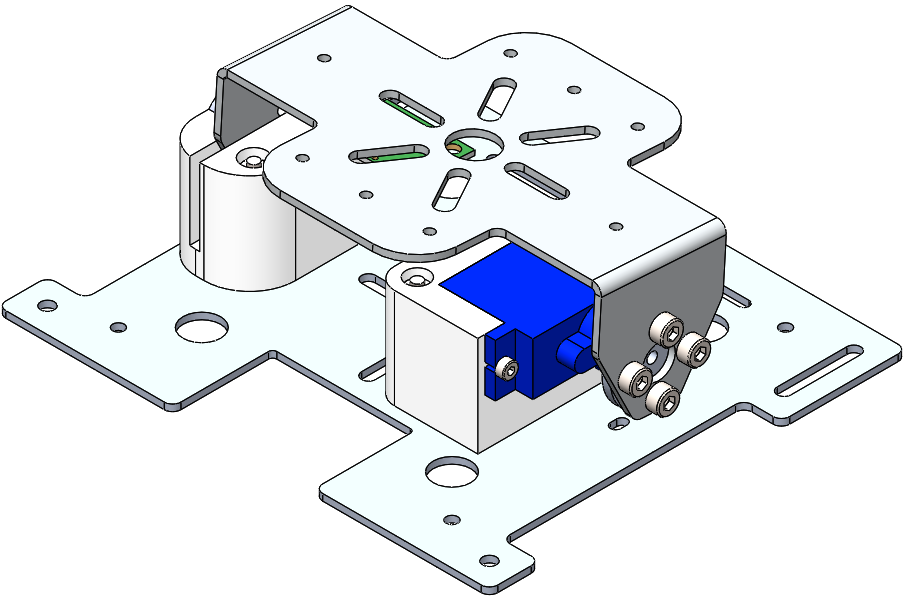
\includegraphics[width = 0.5\textwidth]{Pictures/cover.png}
\end{center}

\newpage
\tableofcontents
\pagenumbering{roman}
\newpage
\listoffigures
\listoftables

\newpage
\pagenumbering{arabic}
\setlength{\parskip}{1em}
\section{Mechanical Design}

The gimbal was designed to stabilize a small camera in one axis. To simplify the construction of the gimbal, a servo motor was used as an actuator and as one of
the two axles for the rotating plate. The servo motor is mounted to a 3D printed mount, which is screwed to a sheet metal plate. Shock absorption balls are used to reduce vibration, and are mounted between two sheet metal plates. To maximize ground clearance to the camera, the gimbal assembly is mounted to the DJI Matrice 100 bottom battery mounting rails. 

\subsection{Sheet Metal Parts}
The three sheet metal parts were designed using Solidworks and made with 1/16'' aluminium cut at the UC Davis ESDC waterjet cutter. The parts are designed to mimic the design and hole layout of the expansion bay plates for the DJI M100, allowing for similar devices to be bolted onto either the expansion plate or the fabricated plates.

\begin{figure}[H]
\begin{centering}
\subfloat[Matrice Plate]{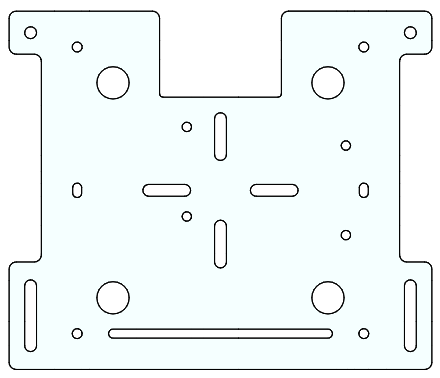
\includegraphics[height = 40mm]{Pictures/matrice_plate.png}} \qquad
\subfloat[Gimbal Plate]{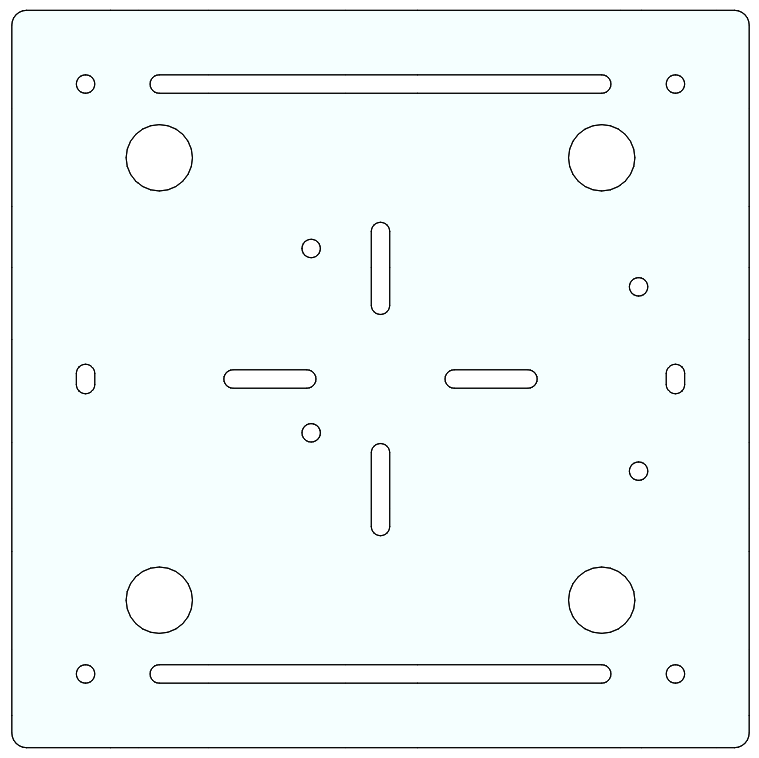
\includegraphics[height = 40mm]{Pictures/gimbal_plate.png}}
\caption{Sheet Metal Plates}
\end{centering}
\end{figure}


\subsection{3D Printed Parts}
3D printed parts were designed with Solidworks and printed at the UC Davis Engineering Student Startup Center. Each file was exported as an .STL file, and processed with slicing software at the ESSC prior to being printed. 

The servo adapter is used to attach the camera plate to the servo motor. The included plastic servo horn is fixed to the servo adapter using 2-part epoxy, with the toothed side of the servo horn facing away from the servo adapter. 




\newpage
\section{Electrical Systems}

The electrical system of the gimbal consists of an Arduino Nano microcontroller mounted to a piece of perforated prototyping board. Tracks on the perforated board distribute power from a 5v output Battery Elimination Circuit (BEC) used to lower the 22v Matrice power output to 5v. Figure \ref{fig:hardware} shows how the various hardware components of the gimbal are connected to one another. 

\begin{figure}[H]
\begin{centering}
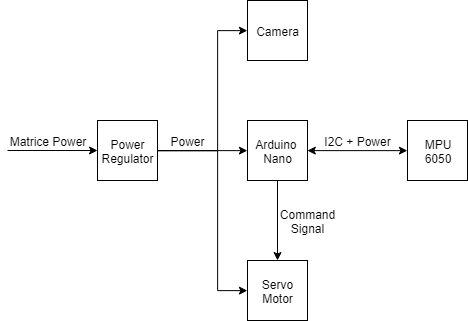
\includegraphics[height = 0.5\textwidth]{Pictures/hardware_flowchart.png}
\caption{Hardware Flowchart}
\label{fig:hardware}
\end{centering}
\end{figure}

\subsection{Microcontroller}
The Arduino Nano microcontroller was chosen to operate the gimbal because of wide software support for Arduino type boards and because its small form factor would allow for convenient mounting on the drone or gimbal. Alternative options such as the Arduino Pro Mini were not used because such boards did not offer USB connectors, and had to be programed with additional FTDI programming chips. 

\subsubsection{Pin Assignments}
The I2C SDA and SCL pins must be connected to pins A4 and A5 respectively due to the hardware of the Arduino Nano, however; the servo output wire can be changed to any arbitrary digital output pin as long as the software is updated to the correct pin.
\begin{table}[H]
	\begin{center}
		\caption{Arduino Nano Pin Assignments}
		\label{tab:nano_pins}
		\begin{tabular}[l]{|c|c|}
			\hline
			\textbf{Pin} & \textbf{Description} \\ \hline \hline
			A4 & MPU6050 SDA  \\ \hline
			A5 & MPU6050 SCL   \\ \hline
			D3 & Servo out wire  \\ \hline
			D13 & Arduino built-in LED \\ \hline
			
		\end{tabular}
		
	\end{center}
\end{table}

\subsection{Inertial Measurement Unit}
An Intertial Measurement Unit is an integrated circuit which can measure orientation and angular velocities. Initially, an MPU9250 was used on the gimbal, however; this was switched to the MPU6050 sensor due to reliability issues with the MPU9250. 

The MPU6050 is a six degree-of-freedom IMU, meaning that there are three acceleration axes and three gyroscope axes. As compared to the MPU9250, which is a nine degree-of-freedom IMU, with three acceleration, gyroscope, and magnetometer axes. While the magnetometer on the 9DOF IMU's can be useful for determining the yaw of the craft in a global reference frame, the one-axis gimbal can function with the 6DOF sensor. 

The MPU6050 communicates via the I2C bus, which allows multiple sensors to be connected along the same two wire bus. The sensitivity of the gyroscope or accelerometer can be separately set by adjusting register values as described in the \href{https://www.invensense.com/wp-content/uploads/2015/02/MPU-6000-Register-Map1.pdf}{MPU6050 Register Map and Descriptions} document. Data is retrieved by reading specific registers allocated to accelerometer/gyroscope data. While the measurements are 16bit integers, the MPU6050 registers are 8bits, with the 16bit measurement split across two registers in Most Significant Bit (MSB) first format, meaning that bits 15 to 8 are stored in the first register, and bits 7 to 0 are stored in the second. To combine these two, shift the first byte ``left'' by 8 bits and perform a logical and with the second byte. 

\subsection{Actuator}
A servo motor was chosen to actuate the gimbal because it allowed for simple control over the angle between the camera plate and the gimbal plate. Unlike brushless DC (BLDC) motors, servo motors do not require special driver circuits to operate, and only require power, ground, and signal connections, however; servo motors have worse resolution when compared to BLDC motors, which limits the effectiveness of the gimbal.

The FMS 9g servo was used because it offered metal gears, which should provide better durability compared to plastic servos, however; the metal gear teeth may erode plastic servo horns, resulting in the camera plate and servo motor decoupling.  


\newpage
\section{Algorithm Design}

The algorithm for running the gimbal can be split into two major sections: the setup procedure and loop process. In the setup procedure, serial communication, I2C communication, the watchdog timer, and the PID class is instantiated. Gyroscope calibration values, PID values, and deadband values are also read from EEPROM memory. The loop process consists of reading data from the Inertial Measurement Unit (IMU), and processing the gyroscope and accelerometer values to yield a pitch angle. The pitch angle is then fed into the PID controller, which determines an output value for the servo. The servo is updated based on this value. The serial buffer is then checked for incoming commands, and the program enters an empty while loop to limit the loop frequency to 180Hz. 

Figure \ref{fig:software_flowchart} represents this chain of operations in a flowchart. 

\begin{figure}[H]
\begin{centering}
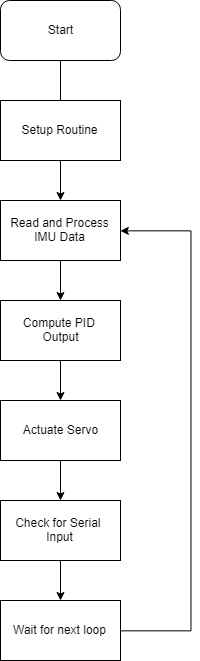
\includegraphics[height = 0.9\textheight]{Pictures/software_flowchart.png}
\caption{Overall Software Flowchart}
\label{fig:software_flowchart}
\end{centering}
\end{figure}

\subsection{Orientation Filter Algorithm}

The core of the gimbal's operation is the algorithm for processing data from the Inertial Measurement Unit (IMU). The key problem lies in combating the main issues regarding the two sensors available: gyroscope readings are precise, but drift over time; accelerometer readings are accurate, but suffer from noise and external forces. To get an accurate and precise measurement of the IMU's orientation, one must use an algorithm that combines data from the two sensors. 

In gimbal firmware 2.2 and below, a simple Euler angle complimentary filter, based on the \href{http://www.brokking.net/imu.html}{work of Joop Brokking},    was used to compute the pitch angle of the IMU. While this approach offered an intuitive approach to processing data, the Euler angle method is susceptible to \href{https://en.wikipedia.org/wiki/Gimbal_lock}{gimbal lock} and suffered from large angle errors when subjected to high non-gravitational accelerations. To address this issue, an adaptive gain quaternion-based complimentary filter was implemented, based on the work of Roberto Valenti, Ivan Dryanovski, and Jizhong Xiao, published in the article \href{http://www.mdpi.com/1424-8220/15/8/19302}{``Keeping a Good Attitude: A Quaternion-Based Orientation Filter for IMUs and MARGs''}. The following section will detail the implementation of this algorithm, and draw comparisons between the Euler angle and Quaternion algorithm.

\newpage
\subsubsection{Implementing the Quaternion-Based Complimentary Filter}
Quaternions are four-element vectors that describe the rotation of objects in 3D space. As opposed to Euler angles, which describe the amount of rotation in the yaw, pitch, and roll axes of a system, three of the four elements in the quaternion define a vector for the axis of rotation, while the fourth, scalar, element defines how much the object is rotated about that axis. Figure \ref{fig:euler_quat} shows how the two types of representation differ. Further details on quaternion orientation representation and mathematical handling can be found \href{http://www.chrobotics.com/library/understanding-quaternions}{here}.
\begin{figure}[H]
\centering
\subfloat[Euler Representation \href{http://www.chrobotics.com/library/understanding-quaternions}{[Source]}]{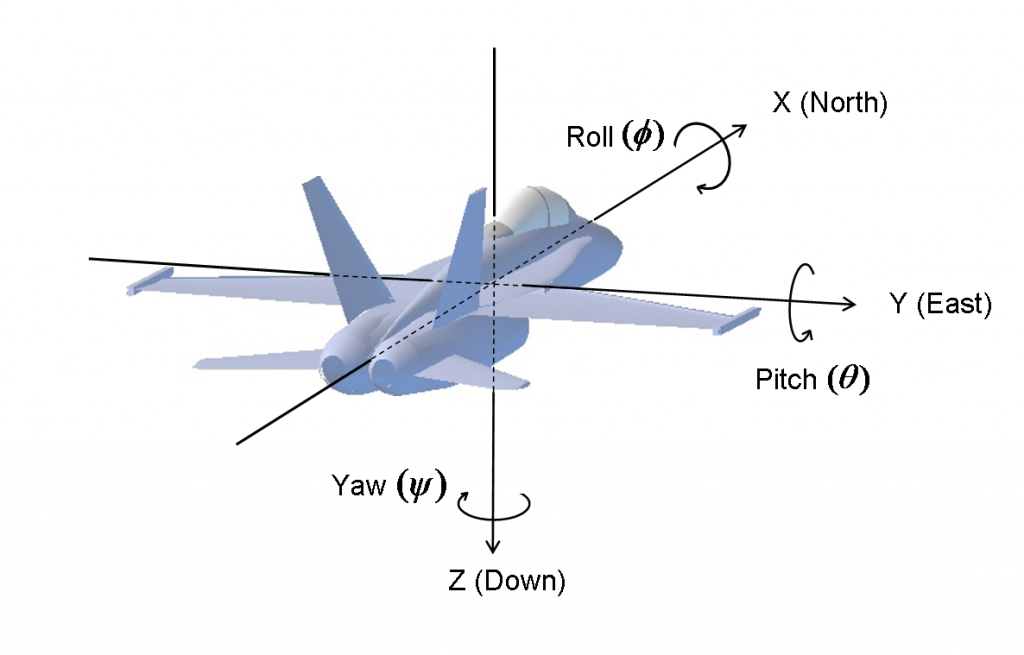
\includegraphics[width = 3.3in]{Pictures/euler.png}}\qquad
\subfloat[Quaternion Representation \href{https://en.wikipedia.org/wiki/Quaternions_and_spatial_rotation}{[Source]}]{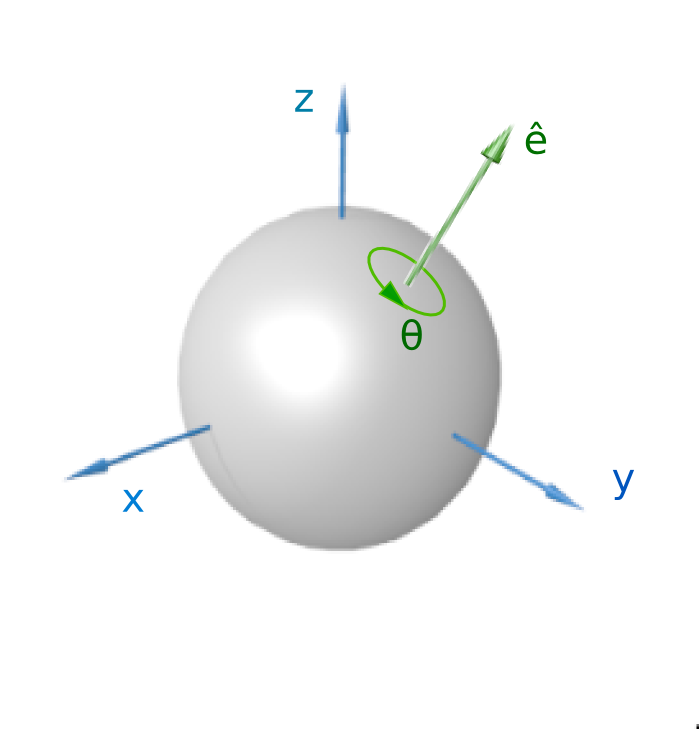
\includegraphics[width = 2.2in]{Pictures/quat.png}}
\caption{Euler and Quaternion Orientation Representation}
\label{fig:euler_quat}
\end{figure}

The algorithm can be split into a number of steps

\begin{enumerate}
	\item Measure IMU and form quaternion $^L\omega_t = [0, \omega_x, \omega_y, \omega_z]$  where $\omega$ represents a reading from the IMU. 
	\item Rotate $^L\omega_t$ from local frame to global frame with previously calculated heading quaternion. \\$-\frac{1}{2}^L\omega_{q,t} \otimes ^L_Gq'_{t-1} = ^L_G\dot{q}_{t-1}$
	\item Integrate numerically to get gyroscope measurement of global frame orientation relative to local frame at time t.\\ $^L_Gq_{\omega, t} = ^L_Gq_{t-1} + ^L_G\dot{q}_{t}\Delta t$
	\item Convert the measured orientation vector to a 3x3 rotation matrix.
	\item Rotate the normalized measured acceleration vector, $^La_t$, by rotation matrix $R(^G_Lq_{\omega,t})$\\
		   $R(^G_Lq_{\omega,t})^La_t = ^Gg_p$, where $^Gg_p$ is the predicted acceleration vector based on the gyroscope estimation. If the gyroscope measurement is completely accurate, the predicted acceleration vector should be $[0,0,0,1]$. 
	\item Because of measurement error and drift, the predicted acceleration vector will likely not be $[0,0,0,1]$. Calculate the rotation quaternion required to rotate $^Gg_p$ vector to $[0,0,0,1]$. \\
		  $\Delta q_{acc} = \Big[\sqrt{\frac{g_z+1}{2}}, -\frac{g_y}{\sqrt{2(g_z+1)}}, \frac{g_x}{\sqrt{2(g_z+1)}}, 0 \Big]$
	\item Run LERP/SLERP complimentary filter on $\Delta q_{acc}$ to yield $\widehat{\Delta q}_{acc}$
	\item Take product of gyroscope orientation quaternion and acceleration compensation quaternion to yield final orientation quaternion.\\
		  $^L_Gq'_t = {^L_Gq_{\omega, t}} \otimes \widehat{\Delta q}_{acc}$
\end{enumerate}

Figure \ref{fig:quat_flowchart} arranges these steps into a flowchart. More detail about the mathematics can be found on pages 19315-19318 of the \href{http://www.mdpi.com/1424-8220/15/8/19302}{``Keeping a Good Attitude''} paper.

\begin{figure}[H]
\begin{centering}
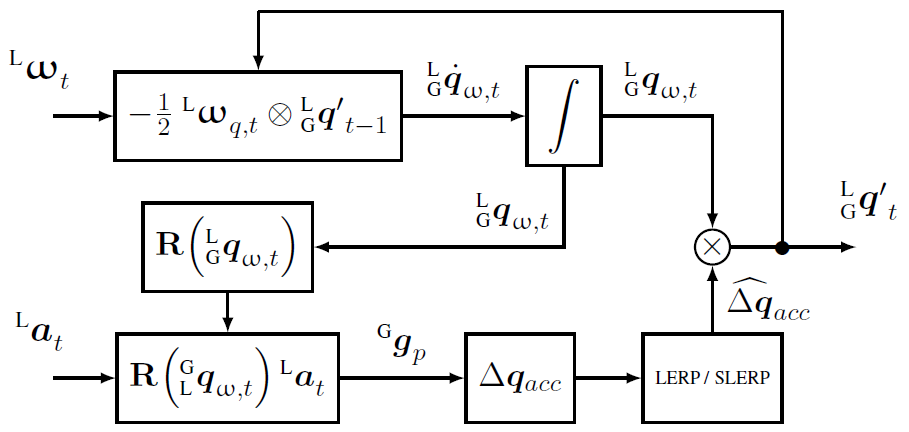
\includegraphics[width = 0.7\textwidth]{Pictures/quat_flowchart.png}
\caption{Quaternion-Based Complimentary Filter Flowchart}
\label{fig:quat_flowchart}
\end{centering}
\end{figure}

\subsubsection{Implementing Adaptive Gain}
While quaternions can resolve issues with gimbal lock (though not actually a concern for a one-axis gimbal), adaptive gain is used to partially resolve issues arising from angle deviations when the IMU is subjected to large, non-gravitational accelerations. Adaptive gain changes the influence the accelerometer has on the final reading, based on a calculated magnitude error. If the error is large, the algorithm will depend heavily on the gyroscope, which is not affected by non-gravitation forces. If the error is small, the algorithm will use both gyroscope and accelerometer readings to combat noise and drift. 

In summary, the adaptive gain function changes the $\alpha$ value dynamically. The value for $\alpha$ can range from 0 to a pre-determined base rate $\bar{\alpha}$ depending on a function that depends on $e_m$, the magnitude of error. 

\[\alpha = \bar{\alpha}f(e_m)\]
\[e_m = \frac{|\|^L\tilde{a}\|-g|}{g}\]

For $e_m$, $\| ^L\tilde{a}\|$ represents the magnitude of the acceleration measured by the IMU in meters per second, prior to being normalized. The function used is a parametric function
\[\begin{cases}
	e_m < L, & 1 \\
	L < e_m < U, & \text{linear between 0 and 1} \\
	U < e_m, & 0 \\
\end{cases}\]
where $L$ is a lower threshold, and $U$ is a upper threshold, both determined experimentally. 

Once again, more details can be found in the \href{http://www.mdpi.com/1424-8220/15/8/19302}{``Keeping a Good Attitude''} paper on page 19320.


\subsection{Testing the Quaternion-Based Filter}

A perfect orientation estimation algorithm would be able to filter out all external non-gravitational forces. In theory, the adaptive gain algorithm should provide performance benefits for orientation estimation. In practice, the adaptive gain can help combat drift when the aircraft is accelerating/decelerating in windy conditions, or when the aircraft is entering/exiting turns. 

To test the resilience of the quaternion-based filter against external non-gravitational forces, an Inertial Measurement Unit (IMU) was placed on a flat surface, and quickly accelerated across the surface. Parameters for base gain, lower threshold, upper threshold, and $\epsilon$ were changed and compared to an Euler estimation algorithm. 

\subsubsection{Varying Base Gain}
Base Gain $\bar{\alpha}$ seemed to have a large impact on the algorithm's performance. Figure \ref{fig:base_gain}  compares the quaternion based algorithm (orange) and Euler angle algorithm (blue) at base gain between 0.01 to 0.05. 
\begin{figure}[H]
\begin{centering}
\subfloat[Base Gain = 0.01]{\includegraphics[width = 0.45\textwidth]{Tests/plots/{0.01-0.05-0.1-0.9}.png}} \qquad
\subfloat[Base Gain = 0.015]{\includegraphics[width = 0.45\textwidth]{Tests/plots/{0.015-0.05-0.1-0.9}.png}} \qquad
\subfloat[Base Gain = 0.017]{\includegraphics[width = 0.45\textwidth]{Tests/plots/{0.017-0.05-0.1-0.9}.png}} \qquad
\subfloat[Base Gain = 0.05]{\includegraphics[width = 0.45\textwidth]{Tests/plots/{0.05-0.05-0.1-0.9}.png}}
\caption{Results of Varying Base Gain}
\label{fig:base_gain}
\end{centering}
\end{figure}
Large base gains can result in the algorithm overshooting, and performing worse than the regular Euler angle algorithm. In contrast, low base gains result in slow compensation and an elongated response. The run performed at base gain = 0.017 performed well, exhibiting less deviation than other trials and recovering sooner than the Euler algorithm.
\newpage

\subsubsection{Varying $\epsilon$}
Changing $\epsilon$ seems to have a similar impact to performance as base gain. Figure \ref{fig:epsilon} compares the quaternion based algorithm (orange) and Euler angle algorithm (blue) at $\epsilon$ between 0.7 to 0.9. 

\begin{figure}[H]
\begin{centering}
\subfloat[$\epsilon$ = 0.7]{\includegraphics[width = 0.45\textwidth]{Tests/plots/{0.017-0.05-0.1-0.7}.png}} \qquad
\subfloat[$\epsilon$ = 0.8]{\includegraphics[width = 0.45\textwidth]{Tests/plots/{0.017-0.05-0.1-0.8}.png}} \qquad
\subfloat[$\epsilon$ = 0.9]{\includegraphics[width = 0.45\textwidth]{Tests/plots/{0.017-0.05-0.1-0.9}.png}}
\caption{Results of Varying $\epsilon$}
\label{fig:epsilon}
\end{centering}
\end{figure}

It seems that larger values of $\epsilon$, around 0.9, perform better than lower values, however; it is interesting that $\epsilon$ = 0.8 performs worse than $\epsilon$ = 0.7. Further testing may be required.

\newpage
\subsubsection{Varying Threshold Values}
Three sets of threshold values were tested. 0.025-0.075, 0.05-0.1, and 0.1-0.2. Figure \ref{fig:threshold} compares the quaternion based algorithm (orange) and Euler angle algorithm (blue) for the three threshold sets.

\begin{figure}[H]
\begin{centering}
\subfloat[L = 0.025, U = 0.075]{\includegraphics[width = 0.45\textwidth]{Tests/plots/{0.017-0.025-0.075-0.9}.png}} \qquad
\subfloat[L = 0.05, U = 0.1]{\includegraphics[width = 0.45\textwidth]{Tests/plots/{0.017-0.05-0.1-0.9}.png}} \qquad
\subfloat[L = 0.1, U = 0.2]{\includegraphics[width = 0.45\textwidth]{Tests/plots/{0.017-0.1-0.2-0.9}.png}}
\caption{Results of Varying Threshold Range}
\label{fig:threshold}
\end{centering}
\end{figure}

It would appear that higher ranges of threshold cause the graph of the quaternion-based algorithm to act like the Euler algorithm. Lower threshold ranges result in smoother, but delayed responses. Further testing may be required to see how the shape of the response curve changes with threshold values. 
 
\subsection{Future Improvements}
Below are a list of possible improvements for the algorithm
\begin{itemize}
\item Use an IMU with a magnetometer to provide compensation along the yaw axis.
\item Test an algorithm with Euler angles and an adaptive gain system to increase algorithm speed.
\item Use a faster microcontroller to increase sampling rate.
\item Continue tuning existing algorithm to improve response and resilience.
	\begin{itemize}
	\item Develop an automated tuner with a gradient descent approach.
	\item Continue further testing on the M100 platform.
	\end{itemize}
\end{itemize}

\section{Arduino Code}

Software for the gimbal was written in Arduino code, which is based on the C++ language, on the Arduino IDE. The code can be uploaded to the Arduino Nano through the Arduino IDE. Files can be found on the \href{https://github.com/DavisDroneClub/gimbal}{Davis Drone Club Github.}
The gimbal code is designed to run on the 16MHz Arduino Nano. Arduino code is based on C and C++, so many resources for C/C++ can be used to understand Arduino code. This section will cover concepts of the code that may not be covered in most learning resources.

\subsection{Union Data Type}

The Union data type is used to store the value of numbers in both float and byte formats. This is useful because the PID and orientation algorithms use data type float for floating point calculations, while the EEPROM data storage requires data in bytes. The Union provides a convenient structure to store both data types under a single variable name. A detailed guide on unions can be found \href{https://www.tutorialspoint.com/cprogramming/c_unions.htm}{here.}

\lstinputlisting[language=Arduino, firstline = 45, lastline = 48]{code/code.ino}

The union is defined in the same way a structure is defined. First use the union statement, followed by the name of the union type. Then in the block enclosed by the brace, include a list of member definitions. In this case, we use float val\_float and byte val\_byte[4] to denote a float value and a 4 byte value (Arduino floats are 32-bit). After the braces, list the names of the variables. In this case we list kp, ki, kd, etc. 

To access the data from a union, use the member access operator (.) by first indicating the variable, followed by the period, and then the desired member definition. For example, kp.val\_float will yield the float value of kp, while kp.val\_byte[0] will yield the first byte of kp. 


\subsection{Reading and Writing EEPROM}

EEPROM is a section of non-volatile memory on the Arduino board, meaning that values stored in EEPROM are not lost when the board is powered off or reset. On the Arduino Nano there are 1024 bytes of EEPROM memory. One consideration when using EEPROM is that EEPROM has limited write cycles. After approximately 100,000 writes, there is a chance that memory will be corrupted or unreadable, however; there are no read limitations for EEPROM memory. Therefore, it is inadvisable to constantly write data the EEPROM. In this case, EEPROM data is only written when certain parameters are changed and read during setup. 

To write to the EEPROM memory, use the EEPROM.h library. The EEPROM.update function further reduces write cycles by checking the value of the memory space first. If the data to be written is the same as the data already present, the memory will not be changed, saving one write cycle. The update function takes two parameters, an index and value. 

More data about the EEPROM library can be found on the \href{https://www.arduino.cc/en/Reference/EEPROM}{Arduino documentation.}

\subsection{Non-Blocking Serial Input}

Non-blocking functions are functions that do not stop the execution of other commands. Non-blocking functions are especially useful for time sensitive programs with functions that take a long time to execute. In this case, reading and writing data to serial takes a considerable amount of time. In firmware version 2.2 and up, the reading functionality is non-blocking, as adapted from the \href{https://hackingmajenkoblog.wordpress.com/2016/02/01/reading-serial-on-the-arduino/}{Majenko Technologies Blog}.


\subsection{Watchdog Timer}

The Arduino Watchdog Timer is a feature to avoid unwanted hangs. The watchdog timer will force the microcontroller to reset if a certain loop timer exceeds a given threshold time. For instance, if a Serial.println() command causes the Arduino to hang, the watchdog timer will automatically reset the Arduino. While the watchdog timer will not help with errors in the implementation of the code, as these errors will occur regardless of how many times the board is reset, the timer is helpful for preventing short term outages, such as issues with power supply or short circuits. 

A useful resource for learning about implementing the watchdog timer can be found \href{https://forum.arduino.cc/index.php?action=dlattach;topic=63651.0;attach=3585}{here.}

\end{document}




